\documentclass[titlepage]{article}

\title{Compiler construction - VYPe15 project documentation}
\author{
	Kidon, Marek\\
	\texttt{xkidon00@stud.fit.vutbr.cz}
\and 
	Janosik, Ondrej\\
	\texttt{xjanos12@stud.fit.vutbr.cz}
}
\date{}

\usepackage[utf8]{inputenc}
\usepackage[IL2]{fontenc}
\usepackage{graphicx}

%\usepackage{mathtools}

\begin{document}
\maketitle

\section{Introduction}
This paper describes the architecture and implementation of the \textit{VYPe15} language
compiler. The compiler itself is implemented in Haskell without any use of compiler 
automatization
tools such as \textbf{lex} \cite{lex}, \textbf{yacc} \cite{yacc} or 
other tools for reasons that will be explained in chapter 
\ref{sec:implementation}. Also the well established concept of 
syntax directed translation was slightly violated.
We will explain why in chapter \ref{sec:architecture}.

\section{Architecture}
\label{sec:architecture}

\subsection{High-level architecture}
In the figure \ref{fig:architecture}, we can see the high-level architecture of our
compiler. As you can see we violated concept of syntax-directed translation.

\begin{figure}[h!]
	\centering
	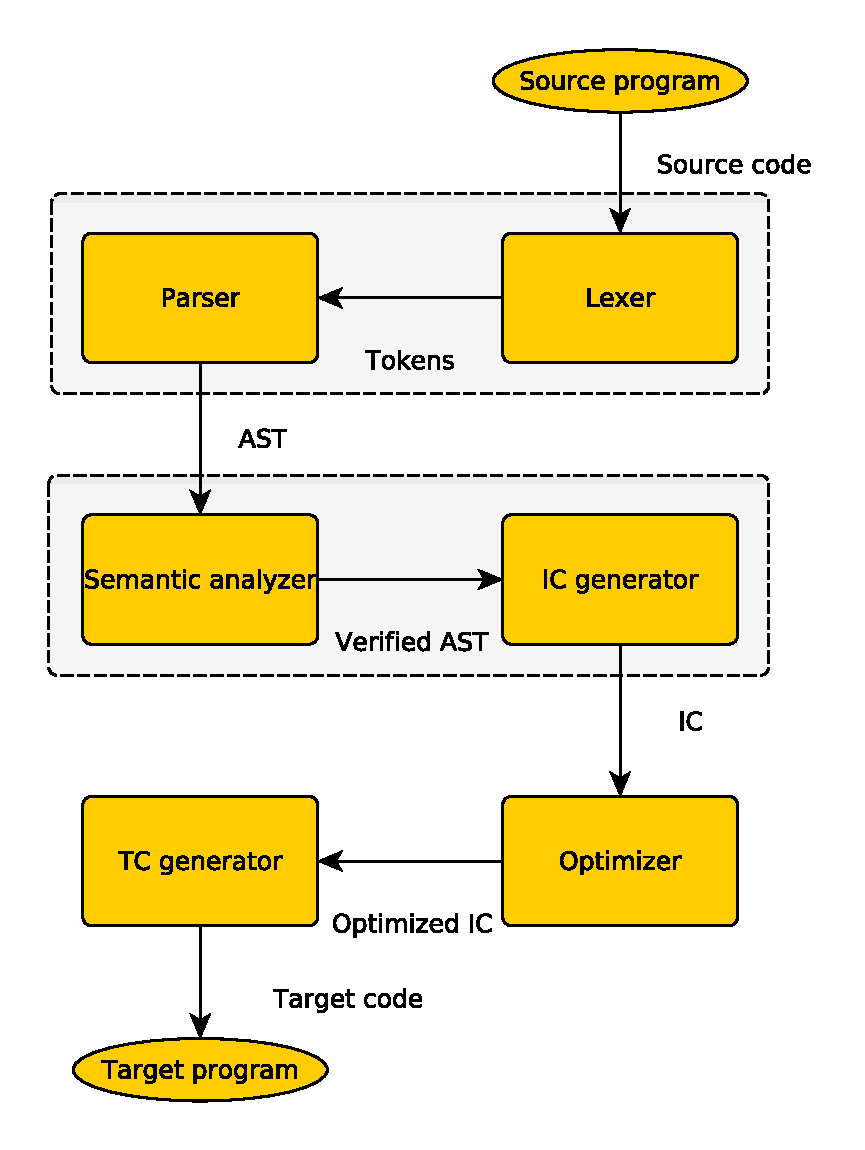
\includegraphics[scale=0.5]{figures/compilerArchitecture}
	\caption{High-level architecture of our compiler.}
	\label{fig:architecture}
\end{figure}

We omitted the semantic analyzer from the syntax analyzer an left it with the intermediate
code generator as a standalone component instead. Numerous reasons lead is to this decision 
such as :

\begin{itemize}
	\item the monadic parser stack would be way too complex to produce reasonable code
		(see chapter \ref{sec:implementation} for further information),
	\item Haskell is lazy-evaluated, so putting semantic analyzer behind the parser does
		not necessarily imply that semantic analysis is performed once parsing is done.
\end{itemize}

The last component is the optimizer/target code generator duo, which is fairly standard.

\subsection{Grammar}
In our parser we implemented the following grammar.

\begin{verbatim}
Program : { FuncDeclr | FuncDef }

FuncDeclr : (DataType | void) Identifier ( TypeParamList ) ;

FuncDef : (DataType | void) Identifier ( ParamList ) '{' { Statement } '}'

DataType : (int | char | string)

TypeParamList : void
			  | DataType {, DataType}
			  
ParamList : void
		  | DataType Identifier {, DataType Identifier}
		  
Statement : Identifier = Expression ;
	      | while '(' Expression ')' '{' {Statement} '}'
	   	  | if '(' Expression ')' '{' { Statement } '}' else '{' { Statement } '}'
	   	  | return ( Expression ; | ; )
	   	  | Identifier '('')' ;
	   	  | Identifier '(' Expression {, Expression} ')' ;
	   	  | DataType Identifier {,Identifier} ;
        
Expression : Expression (|| | && | == | != | < | > | <= | >= | * | /) Expression
           | Expression ( % | + | - | !) Expression
           | (DataType)
           | Identifier
           | Identifier '('')' ;
           | Identifier '(' Expression {, Expression} ')' ;
           | CharLit
           | StringLit
           | NumLit
           
\end{verbatim}


\section{Implementation}
\label{sec:implementation}


\section{Conclusion}
\newpage
\bibliographystyle{alpha}
\bibliography{bibliography}
\end{document}
